\subsection{Reinforcement Learning}
\label{sec::323_rl}
The goal in reinforcement learning is not only to learn actions $a_t$ at time-step $t$, given a state $s_t$, like it is in behavioral cloning, but further to explore actions and states. This is usually performed as shown in figure \ref{fig::323_rl}, where an agent interacts with an environment to receive a reward $r_t$, and also changes the state as cause of its action. Therein, the actions $a_t$ are sampled from a policy $a_t\sim\pi_\theta(a_t|s_t)$ that depends on parameters $\theta$, which for our case are simply the weights of a neural network. 
\begin{figure}[h!]
	\centering
	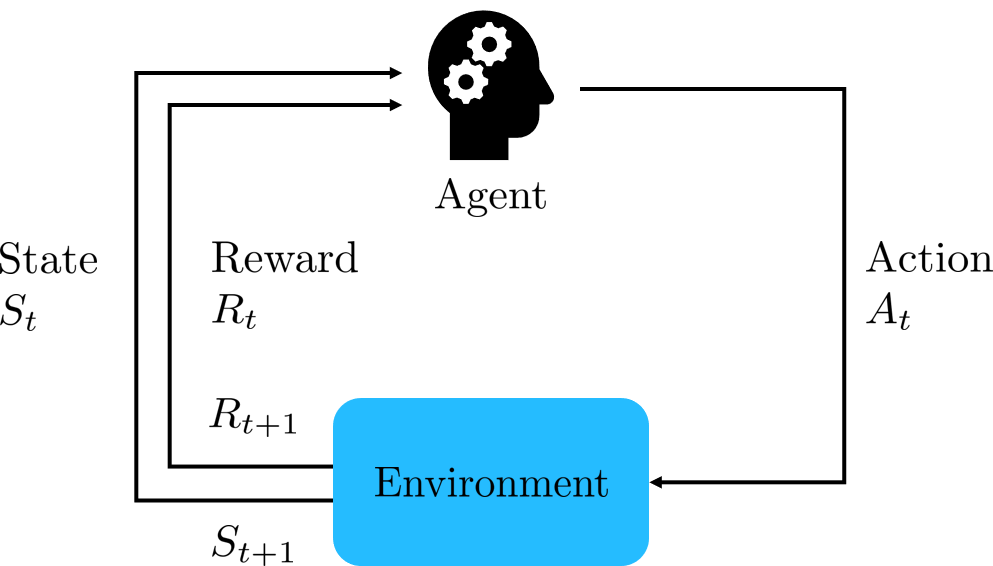
\includegraphics[scale=.5]{chapters/03_background/img/reinforcement_learning.png}
	\caption{Reinforcement learning setup. As the agent interacts with the environment, the state of the environment changes.}
	\label{fig::323_rl}
\end{figure}
The difficulty in optimizing the policy $\pi_\theta$, is to have an agent to discard immediate rewards over future expected rewards. For discrete action spaces, this got well solved by deep Q-learning \cite{mnih2015human}. Different approaches for continuous action spaces like trust region policy optimization \cite{schulman2015trust} are rather complicated. The, to this date, most elegant way of solving continuous control problems in a reinforcement learning setup, is proximal policy optimization \cite{schulman2017proximal}, and we will elaborate on it in the following. Gradient policy methods, such as proximal policy optimization, try to update the policy $\pi_\theta$, such that the expected total future reward $\mathbb{E}\left[\sum_{t=0}^\infty r_t\right]$ is maximized. For the incremental update, it is therefore required to find the gradient of this expression
\begin{align}
	\nabla_\theta\mathbb{E}_{a_t\sim\pi_\theta}\left[\sum_{t=0}^\infty r_t\right] = \mathbb{E}_{a_t\sim\pi_\theta}\left[\sum_{t=0}^\infty\psi_t\nabla_\theta\log\pi_\theta(a_t|s_t)\right],
\end{align}
where $\psi_t$ can take many forms. Since the gradient is just an estimate, as it is computed from samples being taken from the reinforcement learning environment, it usually suffers from variance and bias. As shown in \cite{schulman2015high}, we can trade-off variance for bias and the other way around, by replacing $\psi_t$ for the general advantage estimate $\hat{A}^\text{GAE}_t$ as follows
\begin{align}
	\hat{A}^{\text{GAE}(\gamma,\lambda)}_t = \sum_{l=0}^\infty(\gamma\lambda)^l\delta_{t+l}^V,
	\label{eq::323_gae}
\end{align}
where $\delta^V_{t,l} = r_t + \gamma V(s_{t+1}) - V(s_t)$ is the temporal difference \cite{sutton1998introduction}, and $V$ the value function, which is given by a critic network. The critic's goal then is to have the gradient estimate steer the acting policy network towards actions that maximize the reward. A huge problem therein is that the policy may diverge and that policies may be discarded on the basis of a gradient estimate with a high variance. This is prohibited in proximal policy optimization by clipping the general advantage estimate, and therefore the gradient, under the following objective
\begin{align}
	L^\text{CLIP} = \min(\rho_t(\theta)\hat{A}_t, \text{clip}(\rho_t(\theta), 1-\epsilon, 1+\epsilon)\hat{A}_t),
	\label{eq::323_clip}
\end{align}
where $\rho_t(\theta) = \frac{\pi_\theta(a_t|s_t)}{\pi_{\theta_\text{old}}(a_t|s_t)}$ is the probability ratio of the old and the new policy. The loss is shown in figure \ref{fig::323_ppo}, and it assures for a positive advantage estimate that the gradient does not diverge towards actions that are way more likely under the new policy, than they have been for the old policy.
\begin{figure}[h!]
	\centering
	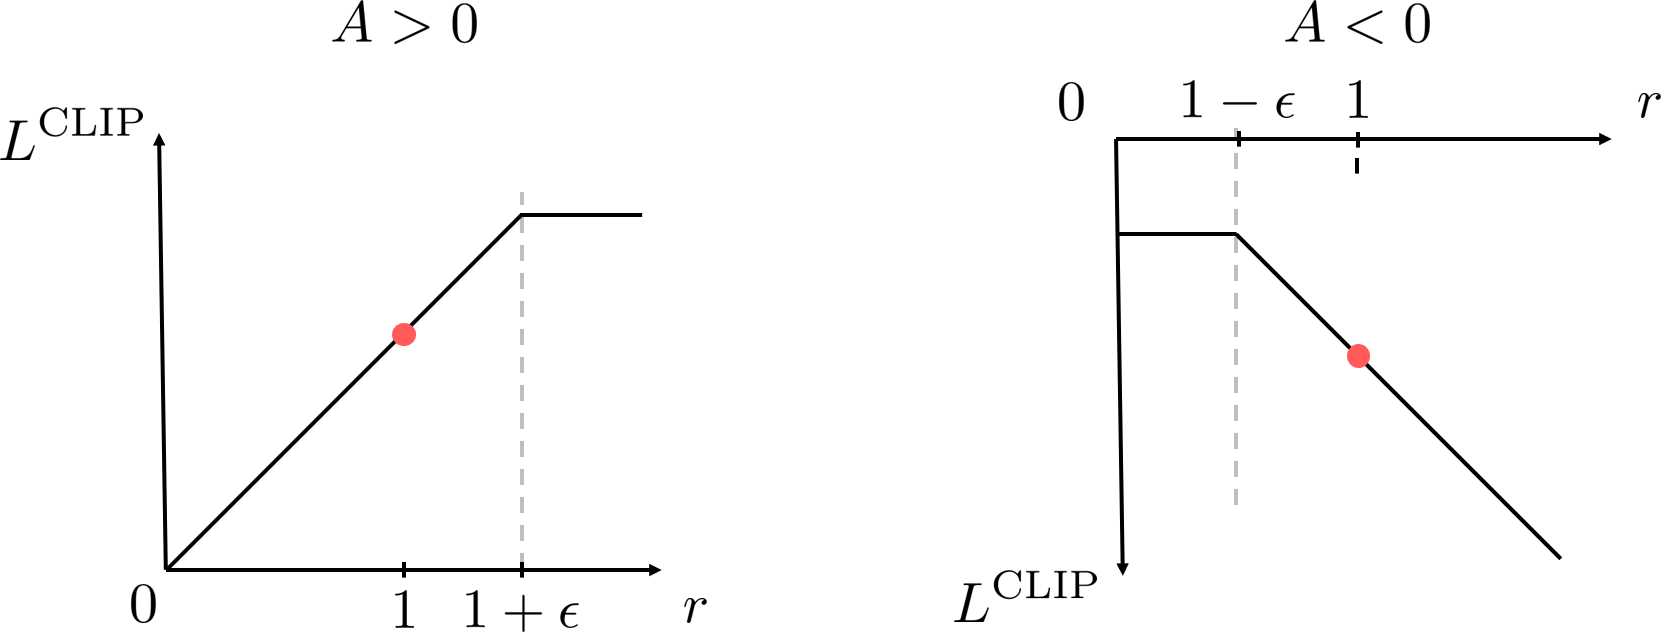
\includegraphics[scale=.35]{chapters/03_background/img/ppo_objective.png}
	\caption{Policy gradient clipping in proximal policy optimization for positive and negative advantage estimates $\hat{A}_t$.}
	\label{fig::323_ppo}
\end{figure}
Also, for a negative advantage estimate, it assures that the gradient points aways from these policies. The total objective $L_t^{\text{CLIP}+\text{VF}+\text{S}}$ of proximal policy optimization is further extended by an entropy term $S$ that results in exploration, and the critic's loss $L^\text{VF}$, such that it can steer the gradient (equation \ref{eq::323_ppo_loss}).
\begin{align}
	L_t^{\text{CLIP}+\text{VF}+\text{S}} = \mathbb{E}\left[L_t^\text{CLIP}(\theta)-c_1L_t^\text{VF}(\theta)+c_2S\left[\pi_\theta\right](s_t)\right]
	\label{eq::323_ppo_loss}
\end{align}
The critic's loss therein is the squared-error of the value function estimate and the explored values $(V_\theta(s_t)-V^\text{target}_t)^2$. The algorithm then runs as follows
\begin{algorithm}
	\SetAlgoLined
	\For{iteration = 1,2,...}{
		\For{runs=1,2,...}{
			Run policy $\pi_{\theta_\text{old}}$ in environment for $T$ timesteps\\
			Compute advantage estimates $\hat{A}^\text{GAE}_1$,...,$\hat{A}^\text{GAE}_T$
		}
		Optimize surrogate $L$ wrt $\theta$, with $K$ epochs and minibatch size $M\leq NT$\\
		$\theta_\text{old}\leftarrow\theta$
	}
	\caption{PPO, Actor-Critic Style}
	\label{alg::325_ac}
\end{algorithm}